\documentclass{article}
%\usepackage{fullpage}

\usepackage[english,french]{babel}
\usepackage[utf8]{inputenc}
\usepackage[T1]{fontenc}

\usepackage{amsmath, amsfonts, amssymb, amsthm}
\usepackage{bbm,algorithmic,algorithm,verbatim}

\usepackage{color}
\usepackage{subcaption}
\usepackage[pdftex]{graphicx}
\usepackage{epsfig}
\usepackage{ulem, stmaryrd, dsfont}

% \usepackage{mathabx} % for \vvvert ||| |||
\usepackage{./tex/sty/scribe}

%%%%%%%%%%%%%%%%%%%%%%%%%%%%%%%%%%%%%%%%%%%%%%%%%%%%%%%%%%%%%%%%%%%%%%%%%%%%%%%
% Hyperlinks

%%%%%%%%%%%%%%%%%%%%%%%%%%%%%%%%%%%%%%%%%%%%%%%%%%%%%%%%%%%%%%%%%%%%%%%%%%%%%%%

\PassOptionsToPackage{hyphens}{url}
\usepackage[pdftex,linkcolor=test,citecolor=vsomb_col,
colorlinks=true,pagebackref,bookmarks=true,plainpages=true,
urlcolor=fb_col]{hyperref}
\usepackage{cleveref}




\begin{document}
\sloppy
\lecture{HMMA307}{REstricted Maximum Likelihood}{Nikolay Oskolkov}{Ophélie Coiffier}


%%%%%%%%%%%%%%%%%%%%%%%%%%%%%%%%%%%%%%%%%%%%%%%%%%%%%%%%%%%%%%%%%%%%%%%%%%%%%%%
%%%%%%%%%%%%%%%%%%%%%%%%%%%%%%%%%%%%%%%%%%%%%%%%%%%%%%%%%%%%%%%%%%%%%%%%%%%%%%%
\section{Introduction}
\label{sec:introduction}
This project speaks about the REstricted Maximum Likelihood (REML).\\
When we calculate a variance estimator with the Maximum Likelihood, we must check if the estimator isn't biased. Actually, in many case, it is biased. The obtained value with the Maximum Likelihood method overestimate (or underestimate) the true value. That's why we need to calculate the variance estimator with REML method.\\
In the first part we will illustrate the issue and we will give an answer to the question :
\begin{center}
    How the REML approach affects the linear mixed model ?
\end{center}
Then, we will mathematically explain and solve the problem.
%%%%%%%%%%%%%%%%%%%%%%%%%%%%%%%%%%%%%%%%%%%%%%%%%%%%%%%%%%%%%%%%%%%%%%%%%%%%%%%
%%%%%%%%%%%%%%%%%%%%%%%%%%%%%%%%%%%%%%%%%%%%%%%%%%%%%%%%%%%%%%%%%%%%%%%%%%%%%%%


%%%%%%%%%%%%%%%%%%%%%%%%%%%%%%%%%%%%%%%%%%%%%%%%%%%%%%%%%%%%%%%%%%%%%%%%%%%%%%%
\section{Illustration of our problem}
In the first part, we illustrate the variance problem with an example. 
\begin{figure}[H]
    \begin{center}
    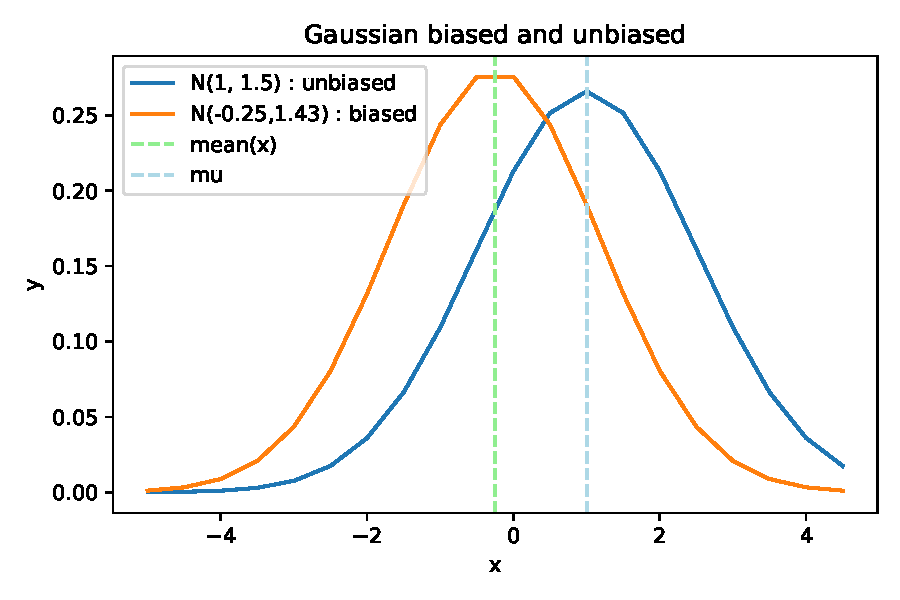
\includegraphics[scale=0.7]{./images/Biased_normal_distri.pdf}
    \caption{Difference between biased Normal distribution and Unbiased Normal distribution.}
    \end{center}
\end{figure}
The Figure 1 shows us the difference between an unbiased Normal distribution and a biased Normal distribution. We see that the mean and the variance are different.\\
Now, we use real data.\\
\begin{table}[h!]
        \centering
        \begin{tabular}{| c | c | c|}
        \hline
        \begin{bf} Ind \end{bf} &
        \begin{bf} Resp \end{bf} &
        \begin{bf} Treat \end{bf} \\
        \hline
        1 &  10 & 0\\
        1 & 25 & 1 \\
        2 & 3 & 0 \\
        2 &  6 & 1\\
        \hline
        \end{tabular}
\end{table}
\textit{Ind} column is the group of the individu, \textit{Resp} column is the treatment response and \textit{Treat} column is an indicator (if the individu gets the treatment, he has 1 else he has 0).\\
The model uses in linear regression is the impact of the treatment on the response.
\begin{equation*}
    Y_{Resp} = \mu +  \alpha X_{Treat} + \varepsilon
\end{equation*}
Where $\varepsilon$ is a noise following a centered, reduced Normal distribution ($\mathcal{N}(0, 1)$).\\
The model uses in linear mixed effects is :
\begin{equation*}
    Y_{Resp} = \mu + \alpha X_{Treat}  + \beta X_{Ind} +\varepsilon
\end{equation*}
When we compare the log-likelihood with both methods, we don't obtain the same result.
With the linear regression, we have $-14.23$ (we can observe this in the Firgure 2, at the point $(8, -14.23)$) while the linear mixed regression (REML) we find $-7.89$.\\
\begin{remark}
\textit{The code is available in the repository called REML but we notice lines we use to show the log-likelihood comparison}
\end{remark}
\begin{lstlisting}
  linear_reg = sm.OLS(df.Resp, df.Treat)
  linear_reg_fit = linear_reg.fit()
  linear_reg_fit.summary()
\end{lstlisting}
\begin{lstlisting}
    mixed_random = smf.mixedlm("Resp ~ Treat", df, groups = df['Ind'])
    mixed_fit = mixed_random.fit()
    mixed_fit.summary() 
\end{lstlisting}
\begin{figure}[H]
    \centering
    \begin{subfigure}[b]{0.7\textwidth}
        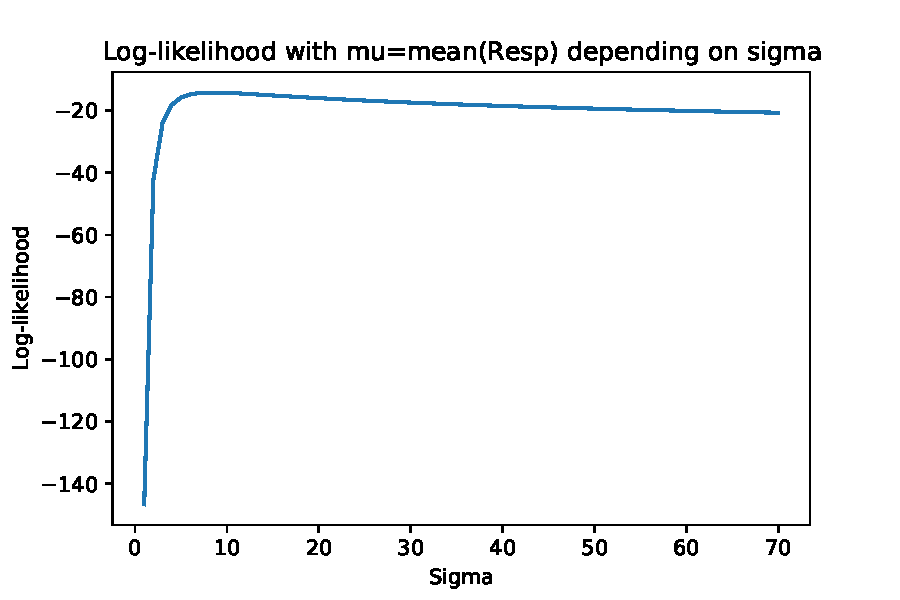
\includegraphics[width=\textwidth]{./images/Log_likelihood.pdf}
    \end{subfigure}
    \begin{subfigure}[b]{0.8\textwidth}
        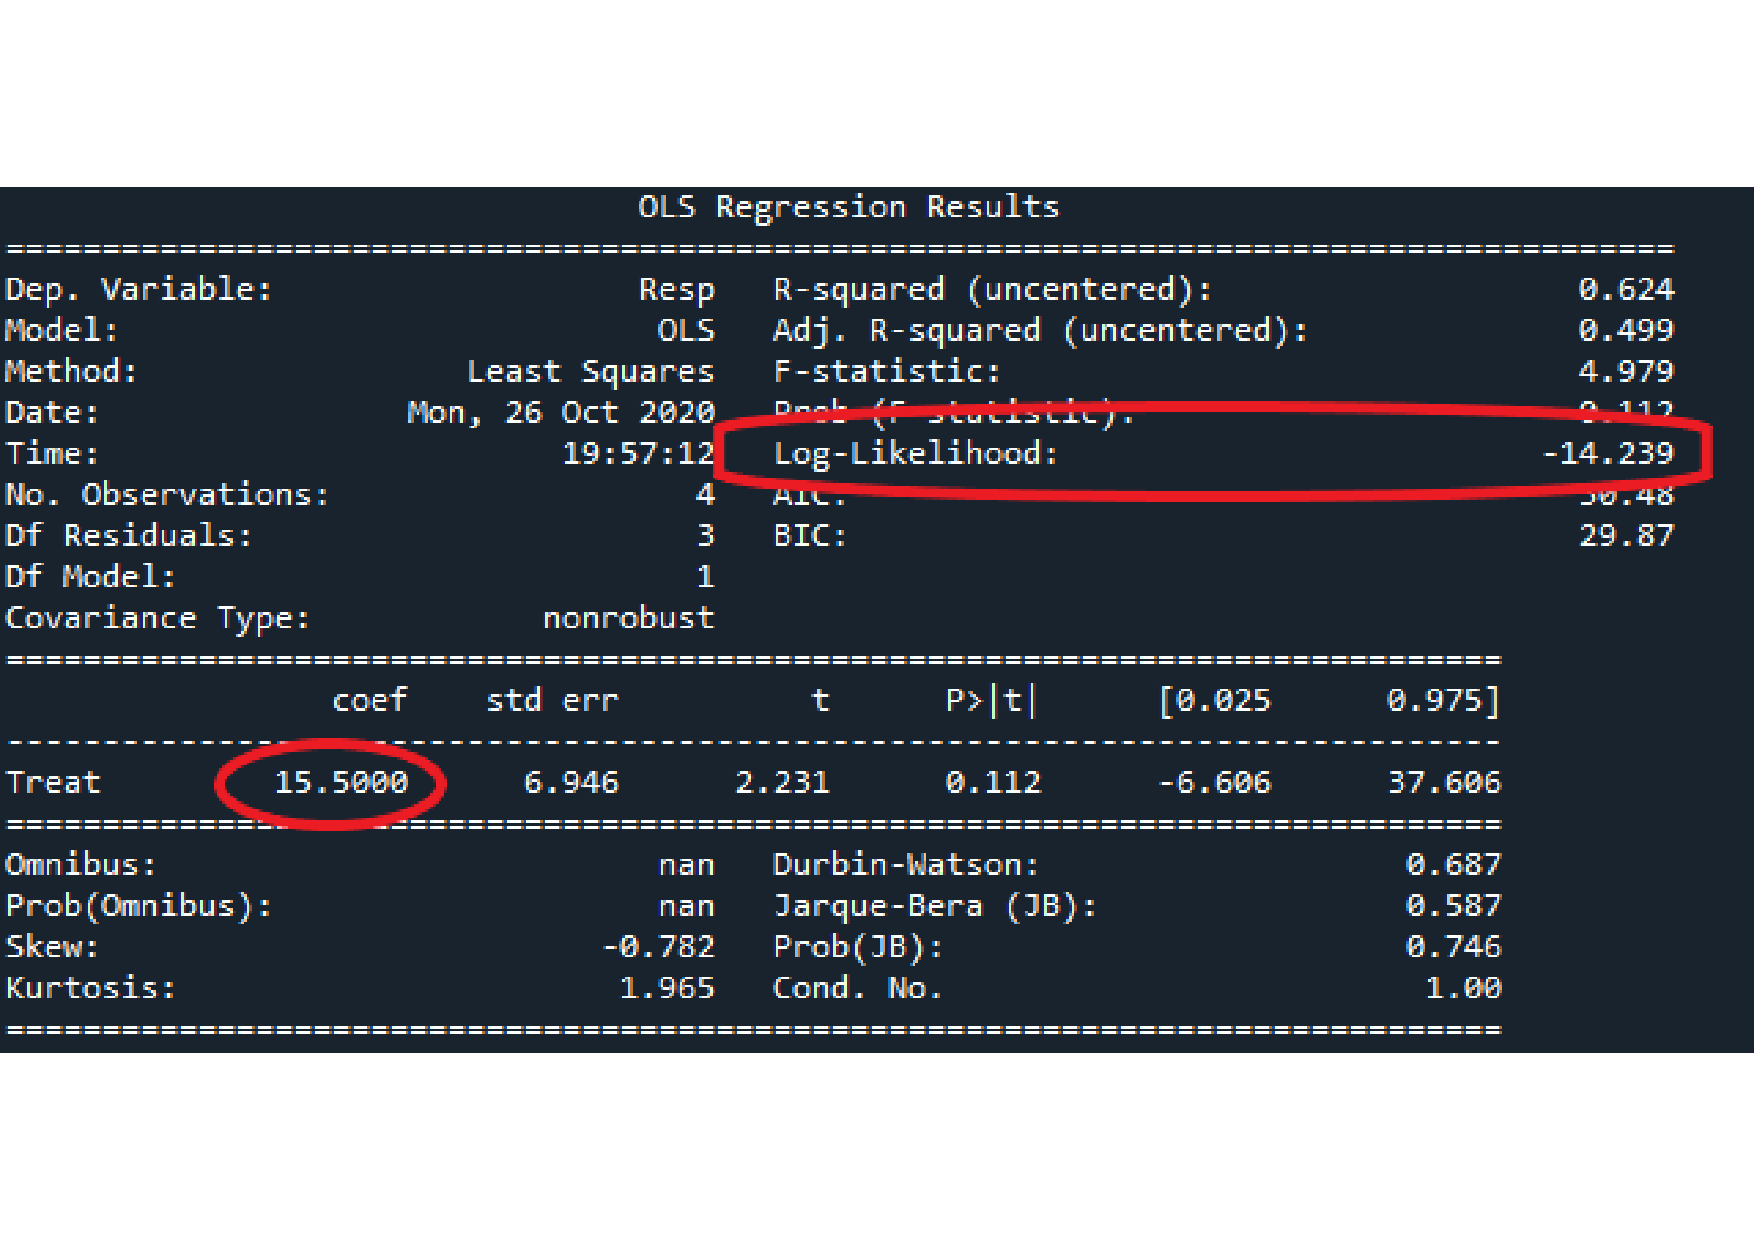
\includegraphics[width=\textwidth]{./images/OLS_Regression.pdf}
    \end{subfigure}
    \caption{The log-likelihood using linear regression depending on $\sigma$ and the result of the linear regression with Python function. }
\end{figure}

\begin{figure}[H]
    \begin{center}
        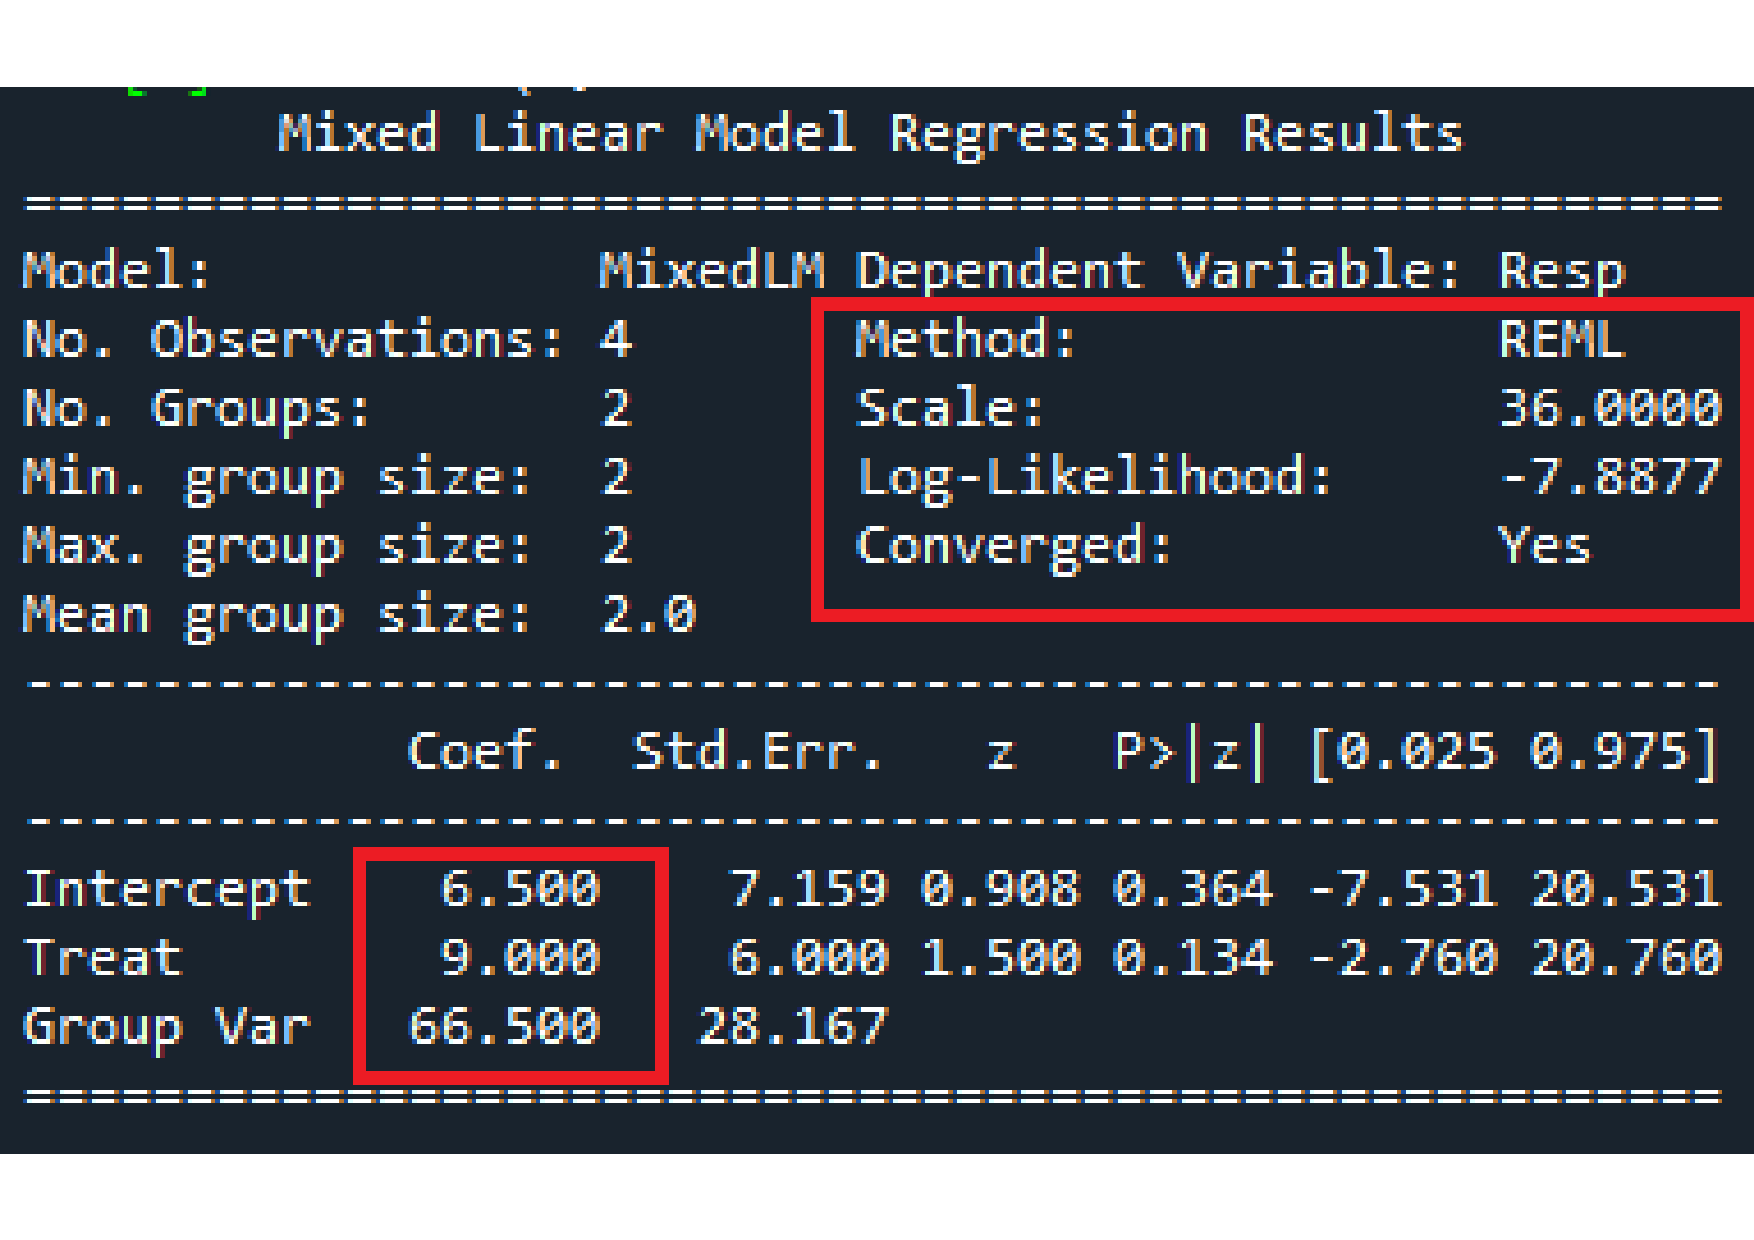
\includegraphics[scale=0.3]{./images/REML_regression.pdf}
        \caption{The log-likelihood using REML regression.}
    \end{center}
\end{figure}
Moreover, we notice the different value of the coefficient : $\sigma^2 =\sqrt{scale}= \sqrt{36.00}= 6.00$\\
$\sigma_s^2 = \sqrt{Group Var}=\sqrt{66.5} = 8.15$, $\beta_1 = 6.0$ and $\beta_2 = (6.5+9.0) = 15.0 = coef.Treat(OLS regression)$\\
Now, we admit the next results and we demonstrate it in the other parts of this report.\\
Thanks to that values, we will compare our results with Python function results.\\
We write out :
\[Y = \begin{pmatrix} 3 & 10 \\ 6 & 25 \end{pmatrix}\]
\[X = \begin{pmatrix} 1 & 0 \\ 0 & 1 \\ 1 & 0 \\ 0 & 1 \end{pmatrix}\]
\[ \Sigma_y = \begin{pmatrix} \sigma^2+\sigma_s^2 & \sigma_s^2 & 0 & 0 \\ \sigma_s^2 & \sigma_s^2+\sigma^2 & 0 & 0 \\ 0 & 0 & \sigma^2+\sigma_s^2 & \sigma_s^2 \\ 0 & 0 & \sigma_s^2 & \sigma_s^2+\sigma^2 \end{pmatrix}\]
\[|\Sigma_y| = 4\sigma_s^4\sigma^4+4\sigma_s^2\sigma^6+\sigma^8\]
\\
Where, $\Sigma_y$ is the variance-covaraince matrix, $|\Sigma_y|$ its determinant.\\
So, we can maximize the integrated log-likelihood (REML purpose, detailed in next part).\\
\textit{The code is available in the Github field (REML.py)}.\\
Actually, we define a function calculates the integrate log-likelihood with two parameters : $\sigma^2$ and $\sigma_s^2$ (doesn't fixed). We know $\beta$ thanks to the linear regression and Y is represented by the \textit{Resp} values. Then, we research the maximum of this function. Our results are the value of $\sigma^2$ and $\sigma_s^2$ which maximize the function.\\
We obtain : $log(\int L(\beta, \Sigma_y)d\beta)=-6.05$, $\sigma_s^2 = 8.15$ and $\sigma^2=6.00$. \\
There are the same results that the values calculating with linear regression.
%%%%%%%%%%%%%%%%%%%%%%%%%%%%%%%%%%%%%%%%%%%%%%%%%%%%%%%%%%%%%%%%%%%%%%%%%%%%%%%

%%%%%%%%%%%%%%%%%%%%%%%%%%%%%%%%%%%%%%%%%%%%%%%%%%%%%%%%%%%%%%%%%%%%%%%%%%%%%%%
\section{The biased variance problem}
When we calculate the maximum likelihood, we transform the likelihood to log-likelihood, then we derive and we equals to zero. And, obviously, we calculate the second derivative of the log-likelihood to check the sign. We need yo have a negative sign to have a maximum.\\
\begin{exemple}
To begin, we calculate the maximum likelihood in $1$ dimension.\\
We take
\[ y = (y_1, \cdots, y_N) \sim \mathcal{N}(\mu, \sigma^2) \]
where $\mu$ is the mean and $\sigma^2$ is the variance.\\
The likelihood is \[ L(y, \mu, \sigma^2) = \prod_{i=1}^N \frac{1}{\sqrt(2\pi \sigma^2)}e^{-\frac{(y_i-\mu)^2}{2\sigma^2}} \]
The log-likelihood is \[l(y, \mu, \sigma^2) = -\frac{N}{2}ln(2\pi\sigma^2)-\sum_{i=1}^N\frac{(y_i-\mu)^2}{2\sigma^2}\]
Now, we derive this function and equals to zero to find the maximum
\begin{equation*}
    \begin{cases}
        \frac{\partial}{\partial \mu}\mid_{\hat{\mu}}l(y, \mu, \sigma^2) = 0 \\
        \frac{\partial}{\partial \sigma^2})\mid_{\hat{\sigma^2}}l(y, \mu, \sigma^2) = 0
    \end{cases}
\end{equation*}
We assure that we have a negative second derivative.\\
Finally, we find \[ (\hat{\mu}, \hat{\sigma^2}) = (\frac{1}{N} \sum_{i=1}^N y_i, \frac{1}{N} \sum_{i=1}^N(y_i-\hat{\mu})^2\]
\end{exemple}
Usually, we stop there, we have our answer but if we calculate the expected value of the variance estimator, we should be obtain the variance estimator (if it's an unbiased estimator).\\
\begin{exemple}
Return at the previous example. We need to know if the variance estimator is unbiased.\\
We write out $\hat{y} = \frac{1}{N} \sum_{i=1}^N y_i = \hat{\mu}$
\begin{equation*}
\begin{split}
   \esp[\hat{\sigma^2}] = \esp[\frac{1}{N} \sum_{i=1}^N(y_i-\hat{\mu})^2] 
   &= \esp[\frac{1}{N} \sum_{i=1}^N(y_i-\mu + \mu - \hat{\mu})^2]\\
   &= \esp[\frac{1}{N} \sum_{i=1}^N((y_i-\mu)^2 + (\hat{\mu}-\mu)^2 - 2(y_i-\mu)(\hat{\mu}-\mu))]
   \end{split}
\end{equation*}
But, we have $\hat{\mu}-\mu = \frac{1}{N}\sum_{i=1}^N y_i-\mu = \frac{1}{N}\sum_{i=1}^N(y_i-\mu)$ \\
So, $\sum_{i=1}^N(y_i-\mu) = N(\hat{\mu}-\mu)$\\
Let's return to our expected value
\begin{equation*}
    \begin{split}
        \esp[\hat{\sigma^2}] = \frac{1}{N} \sum_{i=1}^N \esp[(y_i-\mu)^2]-\frac{2}{N}\esp[N(\hat{\mu}-\mu)^2]+\esp[(\hat{\mu}-\mu)^2] 
        &=  \frac{1}{N} \sum_{i=1}^N\esp[(y_i-\mu)^2]-\esp[(\hat{\mu}-\mu)^2]
    \end{split}
\end{equation*}
We need to find the variance of $(y_i-\mu)$ to continue our calculation.
\[\\Var(y_i-\mu) = \esp[(y_i-\mu)^2]-(\esp[(y_i-\mu)])^2 = \esp[(y_i-\mu)^2] = \sigma^2\]
Finally, we have these equations
\begin{equation*}
    \esp[\hat{\sigma^2}] = \sigma^2 - \esp[(\hat{\mu}-\mu)^2] = \sigma^2 - \Var(\hat{\mu}-\mu) = \sigma^2 - \frac{1}{N^2}\Var(\sum_{i=1}^N y_i) = \sigma^2\frac{N-1}{N} \ne \sigma^2
\end{equation*}
The variance estimator is biased (underestimated the true variance because $\frac{N-1}{N}<1$).To remove the bias, we can change the variance estimator : $\hat{\sigma^2} = \frac{1}{N-1}\sum_{i=1}^N (y_i-\hat{\mu})^2$.
\end{exemple}

We also put these calculations in a higher dimension. In the real life, e.g our illustration, the dimension isn't $1$ but $k$ where $k>1$.
%Faire les calculs en dim k mais pas en exemple pour interpretation
Thanks to these calculations, we see that the maximum likelihood is a good method when $k << N$. But the biased results are obtained when $N\approx k$.\\
That's why, we use the REML method.

%%%%%%%%%%%%%%%%%%%%%%%%%%%%%%%%%%%%%%%%%%%%%%%%%%%%%%%%%%%%%%%%%%%%%%%%%%%%%%%

%%%%%%%%%%%%%%%%%%%%%%%%%%%%%%%%%%%%%%%%%%%%%%%%%%%%%%%%%%%%%%%%%%%%%%%%%%%%%%%
\section{Solve the bias problem}
\begin{exemple}
The main issue is that we use an unknown estimator for the mean. The principle that we will use is : if the log-likelihood has any information about the mean, we can optimize it and find a unbiased variance estimator.\\
\begin{itemize}
    \item First step : integrate the likelihood in relation to $\mu$ and calculate the log of this integration. The parameter $\mu$ will be remove of the equation.
    \item Second step : use Taylor development in the log-likelihood to simplify the formula. 
    \item Third step : separate the formula in $2$ parts (the log-likelihood use in the maximum likelihood and the bias, the REML approach).
    \item Fourth step : finish previous calculations to find the unbiased estimator.
\end{itemize}

\begin{exemple} 
We continue with the previous example (the Normal distribution and $\beta \in \bbR^{2\times 2}$). The likelihood is
\[L(\beta, \sigma_s^2, \sigma^2) = \frac{1}{\sqrt{2\pi |\Sigma_y|}}e^{-\frac{\trans{(Y-X\beta)}\Sigma_y^{-1}(Y-X\beta)}{2}}\]
where $\sigma_s^2$ is random variance effects, $\sigma^2$ is residual effects and $|\Sigma_y|$ is the variance-covariance matrix.\\
First step :
\[log(\int \L(\beta, \Sigma_y)d\beta) = -\frac{1}{2}log(2\pi)-\frac{1}{2}log(|\Sigma_y|)+log(\int e^{-\frac{\trans{(Y-X\beta)}\Sigma_y^{-1}(Y-X\beta)}{2}} d\beta)\]
We write out $f(\beta) = -\frac{\trans{(Y-X\beta)}\Sigma_y^{-1}(Y-X\beta)}{2}$ and we use the Taylor development formula : \\
$f(\beta) \approx f(\hat{\beta}) + \frac{1}{2}(\beta - \hat{\beta})^2f''(\hat{\beta})$\\
Therefore, we obtain :
\[f(\beta) \approx -\frac{\trans{(Y-X\beta)}\Sigma_y^{-1}(Y-X\beta)}{2}-\frac{1}{2}\frac{\trans{(\beta-\hat{\beta})} \trans{X} \Sigma_y^{-1}X (\beta-\hat{\beta})}{2}\]

So, the new log-likelihood is :
\begin{equation*}
    \begin{split}
       log(\int L(\beta, \Sigma_y)d\beta) = -\frac{1}{2}log(2\pi)-\frac{1}{2}log(|\Sigma_y|)+log(\int e^{-\frac{1}{2}\frac{\trans{(\beta-\hat{\beta})} \trans{X} \Sigma_y^{-1}X (\beta-\hat{\beta})}{2} d\beta}) -\frac{\trans{(Y-X\beta)}\Sigma_y^{-1}(Y-X\beta)}{2}\\
       =-\frac{1}{2}log(2\pi)-\frac{1}{2}log(|\Sigma_y|)-\frac{\trans{(Y-X\beta)}\Sigma_y^{-1}(Y-X\beta)}{2} - \frac{1}{2}log(|\trans{X}\Sigma_y^{-1}X|)  
    \end{split}
\end{equation*}
We recognize the solution of the Maximum Likelihood
\[-\frac{1}{2}log(2\pi)-\frac{1}{2}log(|\Sigma_y|)-\frac{\trans{(Y-X\beta)}\Sigma_y^{-1}(Y-X\beta)}{2}\]
And we have the REML approach (the bias) : \[- \frac{1}{2}log(|\trans{X} \Sigma_y^{-1}X|\]
\end{exemple}
In the first part of the document, we have seen an applied example. It shows us how the fee affects the mixed linear model.
\end{exemple}

%%%%%%%%%%%%%%%%%%%%%%%%%%%%%%%%%%%%%%%%%%%%%%%%%%%%%%%%%%%%%%%%%%%%%%%%%%%%%%%

%%%%%%%%%%%%%%%%%%%%%%%%%%%%%%%%%%%%%%%%%%%%%%%%%%%%%%%%%%%%%%%%%%%%%%%%%%%%%%%
%%%%%%%%%%%%%%%%%%%%%%%%%%%%%%%%%%%%%%%%%%%%%%%%%%%%%%%%%%%%%%%%%%%%%%%%%%%%%%%
\section{Deal with linear models in depth}
\label{sec:pour_aller_plus_loin_sur_ce_theme}
%%%%%%%%%%%%%%%%%%%%%%%%%%%%%%%%%%%%%%%%%%%%%%%%%%%%%%%%%%%%%%%%%%%%%%%%%%%%%%%
%%%%%%%%%%%%%%%%%%%%%%%%%%%%%%%%%%%%%%%%%%%%%%%%%%%%%%%%%%%%%%%%%%%%%%%%%%%%%%%
We can read the article and the lesson to learn more about the REML and the linear regression model:
\cite{Google}, \cite{Teaching}

%%%%%%%%%%%%%%%%%%%%%%%%%%%%%%%%%%%%%%%%%%%%%%%%%%%%%%%%%%%%%%%%%%%%%%%%%%%%%%%
\bibliographystyle{alpha}
\bibliography{./biblio/references_all}
%%%%%%%%%%%%%%%%%%%%%%%%%%%%%%%%%%%%%%%%%%%%%%%%%%%%%%%%%%%%%%%%%%%%%%%%%%%%%%%

\end{document}